\chapter{Evaluation}

In this chapter, I will begin by introducing testing problems, against which I will evaluate the implementation. The subsequent section describes the hardware specification of the machines I tested the implementation on. The discussion about the results is in the last section with selected measurements. You can see complete results in appendix chapter \ref{chap:results}. The hyperparameters used for these measurements are in appendix chapter \ref{chap:hyperparameters}.




%%%%%%%%%%%%%%%%%%
%%              %%
%%   PROBLEMS   %%
%%              %%
%%%%%%%%%%%%%%%%%%
\section{Problems description}

For the \acrlong{acc:ga} evolution I used \acrshort{acc:sat} and \acrshort{acc:3sat} problems with various number of literals and clauses. The fitness function sums a number of unsatisfied (for minimization problem) or satisfied (for maximization problem) clauses. I implemented the fitness evaluation in a vectorized manner in PyTorch, so the whole population is evaluated at once. I generate a new problem for every new measurement, and all the problems have been satisfiable. I achieved that by generating the first assignment of all the literals and then generating the desired number of clauses. At least one literal in each clause matches the value with his corresponding counterpart in the previously generated assignment. Because I am more concerned with the running time of the algorithm rather than its performance, the satisfiability of the formulas does not make a big impact on the measurements.

The problem formula is kept as a matrix, where rows correspond to clauses and columns to indices of literals in the clause. For a negative literal, the index is negative. This coding is efficient for \acrshort{acc:3sat} problem, but I run into a problem with generic \acrshort{acc:sat} problem with a diverse number of literals in the clause. Because the tensors in PyTorch need to be aligned in each dimension, I transform the generic \acrshort{acc:sat} problem into $k$-SAT problem, where $k$ is equal to the length of the longest clause. The shorter clauses duplicate their first literal, so their truth evaluation does not change, and the clause has exactly $k$ literals. This may lead to a considerable inefficiency if the length variance between clauses is high. It may be worth divide long clauses into smaller ones to reduce the overall size of the tensor and save some memory and computation. I believe this is not a serious obstacle for a broader application of the implementation.

The implementation process files in the \textit{DIMACS CNF} format, which is the general and standard file format to define Boolean expression written in conjunctive normal form \citep{challenge1993satisfiability}. The evaluation and parser implementation, with the script to generates the problems, are in the attachment.

For the \acrlong{acc:pso} and real--coded evolutionary algorithms I used well--established \acrfull{acc:coco} \acrfull{acc:bbob} test suite \citep{hansen2010comparing}. The suite consists of $24$ functions in $5$ groups with increasing difficulty. The groups vary in their separability, conditioning, unimodality, and global structure. It would not be feasible for me to measure the algorithm on all of them. Furthermore, as I am more interested in the algorithm's running time, there is no need to evaluate the implementation on all of them. The shifts in the running time would be caused primarily by the speed of the function evaluation rather than the algorithm itself.

The functions are randomly shifted in the search space. The $\mathbf{x}^{opt}$ specifies the position of the optimum. The optimum is always kept in the $\left[-5,5\right]$ interval in each dimension. Moreover, to eliminate the dependency of the algorithm on the absolute value of the function, it is shifted by the $f_{opt}$ value sampled from the Cauchy distribution with zero mean and scale equal $100$. This makes it difficult to directly use proportional--based selection operators because the optimum value differs each run and may be even negative. The algorithm does not know the $\mathbf{x}^{opt}$ and $f_{opt}$ values, and these are only used for the measurements. Except $\mathbf{x}^{opt}$ and $f_{opt}$, the functions may have other parameters (typically rotation matrices $\mathbf{R}$ and $\mathbf{Q}$, or diagonal scaling matrix $\Lambda$), that I will not describe here. You can see the exact definition in the \acrshort{acc:bbob} specification \citep{hansen2010comparing}. These parameters are initialized randomly before each run. Lastly, the functions allow to specify their dimension $D$ at runtime, and the parameters are initialized accordingly. It is, therefore, easy to evaluate the algorithm on the same function with a different number of dimensions and hence on the problem with different difficulty.

I chose the following functions to evaluate the implementation. Not all the aspects of the algorithms were tested on all of these functions.
\begin{itemize}
    \item Function $f_1$ -- sphere function, that is unimodal, highly symmetric, rotationally and scale invariant. Sphere function is probably the simplest one, and can be easily solved using local search techniques.
    \begin{align*}
        f_{1}\left(\mathbf{x}\right) &= \norm{\mathbf{z}}^2+f_{opt} \\
        \mathbf{z} &= \mathbf{x} - \mathbf{x}^{opt}
    \end{align*}
    \item Function $f_7$ -- step ellipsoidal function. This function is unimodal, non--separable and has low conditioning. Because of the step nature of the algorithm, it has many plateaus with zero gradient, so the gradient--based methods would not be very successful. Nevertheless, the function still exhibit ellipsoidal shape. 
    \begin{align*}
        f_{7}\left(\mathbf{x}\right) &= 0.1\max\left( \frac{\abs{\hat{z}_1}}{10^4}, \sum_{i=0}^D 10^{2\frac{i-1}{D-i}}z_i^2 \right) + f_{pen}\left( \mathbf{x} \right)+f_{opt} \\
        \hat{\mathbf{z}} &= \Lambda^{10}\mathbf{R} \left( \mathbf{x} - \mathbf{x}^{opt} \right) \\
        \tilde{z}_i &=\left\{ 
            \begin{array}{ll}
                \lceil 0.5 + \hat{z}_i \rceil       & \text{if}\ \hat{z}_i>0.5 \\
                \lceil 0.5 + 10\hat{z}_i\rceil / 10 & \text{otherwise}        \\
            \end{array}  
            \right. \\
        \mathbf{z} &= \mathbf{Q}\mathbf{\tilde{z}} 
    \end{align*}
    \item Function $f_{15}$ -- Rastrigin function, that is non--separable, have roughly $10^D$ local optimima, low conditioning and local amplitude large compared to local amplitudes. The function is highly multimodal and is not symetric or regular.
    \begin{align*}
        f_{15} &= 10\left( D-\sum_{i=1}^D \cos\left(2 \pi z_i\right) \right) + \norm{\mathbf{z}}^2+f_{opt} \\
        \mathbf{z} &= \mathbf{R}\Lambda^{10}\mathbf{Q}T_{asy}^{0.2} \left( T_{osz}\left(\mathbf{R}\left(\mathbf{z}-\mathbf{x}^{opt}\right)\right) \right)
    \end{align*}
    \item Function $f_{19}$ -- composite Griewank--Rosenbrock function. This function is highly multimodal and noisy.
    \begin{align*}
        f_{19}\left(\mathbf{x}\right) &= \frac{10}{D-1}\sum_{i=1}^{D-1}\left( \frac{s_i}{4000} - \cos\left(s_i\right) \right) + 10 + f_{opt}\\
        \mathbf{z} &= \max\left(1,\frac{\sqrt{D}}{8}\right)\mathbf{R}\mathbf{x}+0.5 \\
        s_i &= 100 \left(z_i^2 - z_{i+1}\right)^2 + \left(z_i-1\right)^2 \\
        \mathbf{z}_{opt} &= \mathbf{1}
    \end{align*}
    \item Function $f_{22}$ -- Gallagher's Gaussian 21--hi peaks function with 21 unrelated and random optimas.
    \begin{align*}
        f_{22}\left(\mathbf{x}\right) &= T_{osz}\left( 
            10 - \max_{i=1}^{21} w_i \exp\left( -\frac{1}{2D}\left(\mathbf{x}-\mathbf{y_i}\right)^T\mathbf{R}^T\mathbf{C}_i\mathbf{R}\left(\mathbf{x}-\mathbf{y_i}\right) \right) 
        \right)^2 + \\
        & + f_{pen}(\mathbf{x}) + f_{opt} \\
        w_i &= \left\{
            \begin{array}{ll}
                1.1+8\frac{i-2}{19} & \text{for}\ i=2,\dots,21 \\
                10                  & \text{for}\ i=1 \\
            \end{array}
        \right.
        \\
        \mathbf{C}_i &= \Lambda^{\alpha_i} / \sqrt[4]{\alpha_i} \\
        \alpha_i &= \left\{ 
            \begin{array}{ll}
                \alpha_i = 10^6 & 
                    \begin{array}{l}
                        \text{for}\ i=1
                    \end{array} \\
                \alpha_i \in \left\{1000^{2\frac{j}{19}}|j=0,\dots,19\right\} &
                    \begin{array}{l}
                        \text{sampled randomly without} \\
                        \text{replacement for}\ i \neq 1
                    \end{array}
            \end{array}
        \right.
    \end{align*}
    \item Function $f_{24}$ -- Lunacek bi--Rastrigin function. This function is highly multimodal and deceptive, because of the promising area with local optima.
    \begin{align*}
        f_{24}\left(\mathbf{x}\right) &=
            \min\left( \sum_{i=1}^D\left(\hat{x}_i-\mu_0\right)^2, dD+s\sum_{i=1}^D\left(\hat{x}_i-\mu_1\right)^2 \right) + \\
            &+ 10\left(D-\sum_{i=1}^D \cos\left(2\pi z_i\right)\right)
            + 10^4 f_{pen}\left(\mathbf{x}\right) \\
        \hat{\mathbf{x}} &= 2 \text{sign}\left(\mathbf{x}^{opt}\right) \bigotimes \mathbf{x} \\
        \mathbf{x}^{opt} &= \mu_0 \mathbf{1}^{+}_{-} \\
        \mathbf{z} &= \mathbf{Q}\Lambda^{100}\mathbf{R}\left(\hat{\mathbf{x}}-\mu_0\mathbf{1}\right) \\
        \mu_0&=2.5,\mu_1=-\sqrt{\frac{\mu_0^2-d}{s}}, s=1-\frac{1}{2\sqrt{D+20}-8.2},d=1
    \end{align*}
\end{itemize}

I reimplement all the \acrshort{acc:bbob} functions in PyTorch. They are fully vectorized so that the whole population can be evaluated at once. The implementation of these functions is in the attachment and is also available from PyPI as the \href{https://pypi.org/project/BBOBtorch/}{\textit{BBOBtorch}} package.




%%%%%%%%%%$%%%%%%%
%%              %%
%%   HARDWARE   %%
%%              %%
%%%%%%%%%%%$%%%%%%
\section{Hardware specification}

I run all my experiments in \href{https://metavo.metacentrum.cz/en/}{MetaCentrum}. For workloads running on \cpu I used servers with specification in table \ref{tab:cpuspec}. For \gpu specialized tasks, I used servers with hardware specified in table \ref{tab:gpuspec}.


\begin{table}[t]
    \begin{subtable}[b]{0.4\textwidth}
        \begin{tabular}[b]{|l|l|}
            \hline
            CPU     &   AMD EPYC 7452 \\
            \hline
            RAM     &   $256$ GiB \\
            \hline
            Disk    &   $2\times4$ TB HDD \\
            \hline
            Owner   &   \makecell{Faculty of Science,\\Charles University} \\
            \hline
        \end{tabular}
        \caption{Hardware specification for \acrshort*{acc:cpu} measurements}
        \label{tab:cpuspec}
    \end{subtable}
    \hfill
    \begin{subtable}[b]{0.55\textwidth}
        \begin{tabular}[b]{|l|l|}
            \hline
            CPU     &   Intel\textsuperscript{\textregistered} {X}eon\textsuperscript{\textregistered} Gold 5218 \\
            \hline
            RAM     &   $192$ GiB \\
            \hline
            Disk    &   $4\times240$ GB SSD \\
            \hline
            GPU     &   nVidia Tesla T4 \\
            \hline
            GPU memory     &   16GB \\
            \hline
            \cuda cores     &   2560 \\
            \hline
            Tensor cores     &   320 \\
            \hline
            Owner   &   CESNET \\
            \hline
        \end{tabular}
        \caption{Hardware specification for \acrshort*{acc:gpu} measurements}
        \label{tab:gpuspec}
    \end{subtable}
    \caption{Hardware specification of server implementation was tested on}
\end{table}

One drawback of using MetaCentrum is that the machines are shared amongst the academic community of the Czech Republic. I could not block the whole machine for a more extended time, principally because it would not be morally correct. I have done all the \cpu workloads using tasks with eight cores and all the \gpu workloads with two cores.

While some of the resources, for example \gpu and RAM, are allocated exclusively to the running task, other, for example disk, network bandwidth, and \cpu to some extent, are not. The \cpu situation is further complicated by the Hyper--Threading technology. This technology duplicates one physical processor core into two logical ones. While the first may use the full utilization of the core, the second one uses the idle portion of it. All the processors currently installed in the MetaCentrum, including the AMD EPYC 7452 processor, dispose this technology. As the goal of this work is focused on the computation quantity rather than on the raw computation power, measurements done on this second logical core may have a significant impact on the execution time, especially for the \cpu workloads. I did my best to mitigate this issue by allocating extra cores, running the measurements during unoccupied hours, and running the measurements on the same machine so that no other user could interfere. Nevertheless, the measurements may still be noisy.




%%%%%%%%%%%%%%%%%
%%             %%
%%   RESULTS   %%
%%             %%
%%%%%%%%%%%%%%%%%
\section{Results discussion}

I run all the experiments on the hardware specified above, and because the \acrlong{acc:ea} are by their nature stochastic, I repeated each experiment a hundred times. The reported numbers are the mean of the given metric over these runs.

\definecolor{superlightgray}{gray}{0.92}
\vskip\baselineskip\noindent\colorbox{superlightgray}{\begin{minipage}{0.98\textwidth}
\leavevmode{\parindent=1em\indent} First \cuda call from the PyTorch runtime initialize the \cuda context and based on my measurements, it takes about $1.5$s. The initialization is done only once during the execution of the Python script and could add bias to the first run of the algorithm. I decided not to take the delay into account, and all the measurements in this work are without it. I would argue this delay is spread over the runs, and because of the stochastic nature of the \acrshort{acc:ea}, they should be executed multiple times in order to get reliable results.
\end{minipage}}
\vskip\baselineskip

The experiments run in the most cases for the population of sizes $32$, $128$, $200$, $512$, $1024$, $2048$, $5000$, $10240$, $16384$, and $32768$. These values play a role in all the experiments and, most of the time, are the quantity shown on the $x$ axis.

Based on the experiments, the \cuda implementation seems to perform better from medium to big--sized problems and populations. That is not surprising, as the \gpu is intended for vast computation and memory demands. For small problems and populations, the runtime stays constant up to a certain threshold, where the runtime starts to increase linearly with the problem size. This is clearly visible in figure \ref{meas:garuntime} for \acrshort{acc:3sat} problem with $100$, $300$, and $800$ literals. In the case of $2000$ literals, I would already classify the problem as medium-sized. The time for even the smallest population of $32$ individuals is the same for both \cpu and \gpu implementation. Measurement of \acrshort{acc:3sat} problem with varying number of literals and clauses is depicted in figures \ref{meas:garuntimeproblemsize} and the \gpu implementation clearly outperform the \cpu one over the whole domain. Note that I used a population size of $1000$ individuals, which is advantageous for the \gpu implementation.

\begin{figure}
    \begin{subfigure}[t]{0.45\textwidth}
        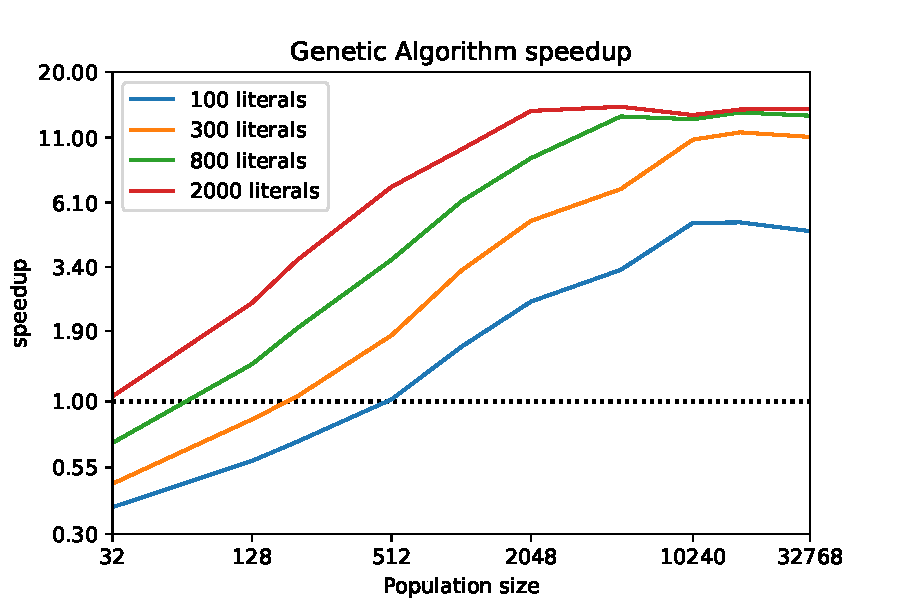
\includegraphics[width=\textwidth]{img/runs/speedup_ga.pdf}
        \caption{Speed up of \acrshort*{acc:ga} on \acrshort*{acc:gpu}}
        \label{fig:gpugaspeedup}
    \end{subfigure}
    \hfill
    \begin{subfigure}[t]{0.45\textwidth}
        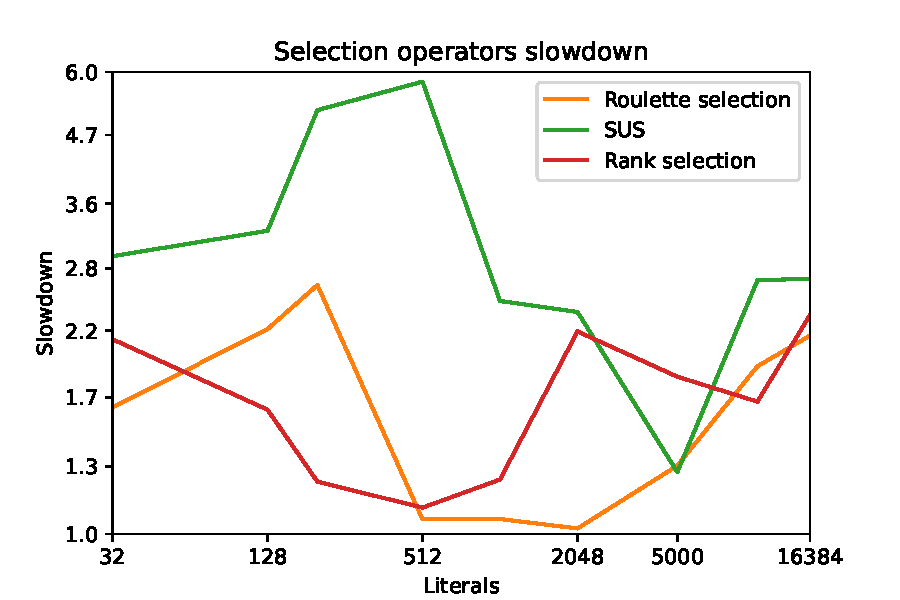
\includegraphics[width=\textwidth]{img/runs/time_ga_selection_slowdown.pdf}
        \caption[Slowdown of GA selection operators]{Slowdown of \acrshort*{acc:ga} on \gpu with various selection operators in constrast to tournament selection}
        \label{fig:gpugaselectionslowdown}
    \end{subfigure}

    \caption{\acrlong*{acc:ga} evaluation}
\end{figure}

The interesting observation is the constant run time of the \gpu implementation for small populations and problems. In these cases, the \gpu is not fully utilized, and the whole population can be processed truly in parallel. As the \cuda cores are less performant than \cpu cores, the total running time is higher than of \cpuns. Moreover, the communication overhead between \cpu and \gpu plays a relevant role in the running time. The speedup of the algorithm running on the \gpu is depicted in figure \ref{fig:gpugaspeedup}.

I compared the PyTorch implementation to \cpp one in figure \ref{meas:cimpl}. You can find the \cpp implementation in the attachment. It used master--worker architecture, where the fitness evaluation is done in parallel using multiple cores, whereas the rest of the algorithm is sequential. Both implementations use the same hyperparameters specified in chapter \ref{chap:hyperparameters}. I compared the implementation using one and eight cores, along with the \gpu implementation. You may notice that \cpp implementation using one core outperforms PyTorch implementation by around $80\%$. Python is an inherently slow language, and the additional overhead of calling native code from Python underlines it. Moreover, the PyTorch implementation is a bit complicated compared to simple \cpp implementation, which may also influence the running time. When I compared the implementations using eight cores, the difference is almost negligible (around $20\%$). The PyTorch implementation took advantage of the parallelization of all the operators, and I believe an increased number of cores would further favor PyTorch implementation. The \gpu implementation still outperforms the \cpp implementation in order of magnitude on populations larger than two thousand individuals.

Of course, one would use a larger population only if it is advantageous. I measured the progress of fitness value over the generation, and these experiments are depicted in figure \ref{meas:gafitness} and \ref{meas:gafitnesselite} (with elitism). I measured the $0.05$ quantile of the fitness function, and the algorithm converges increasingly faster for populations of size $32$, $512$, and $5000$. The big populations with $10240$ and $32768$ individuals do not make an impact until solving big enough \acrshort{acc:3sat} problem with $2000$ and $5000$ literals. Unfortunately, the improvement is not as significant as between the populations of size $512$ and $5000$. In my opinion, using that big population for this kind of problem is not worth it.

Running time of various selection operators in \acrshort{acc:sat} problem is in figure \ref{meas:selection}. Note that this is one of the more noisy experiments, although I repeat the experiment multiple times. For the \cpu implementation, the fitness evaluation is the operator taking most of the time, and the impact of the selection operator is scant. On the \gpu is the situation different, and the selection operators seem to have an order of magnitude difference. The fastest one is the tournament selection, which is not surprising, as it does not require sorting or search in the fitness array in any way. On the other hand, the \acrshort{acc:sus} seems to be the slowest of them, especially for smaller populations. For bigger populations of the size greater than $5000$ the performance of roulette, \acrshort{acc:sus} and rank selection look very similar. You can see the slowdown of these operators in comparison to tournament selection in figure \ref{fig:gpugaselectionslowdown}. As you may notice, the measurements are unfortunately very noisy.

Lastly, I measured the impact of fitness scaling operators on the run time of the \acrshort{acc:ga}, and these results are in figure \ref{meas:scale}. The algorithm used tournament selection, and the different scale operators did not influence the algorithm's performance. Similarly to the selection, the fitness evaluation took the longest time, and the execution of the scale function does not make any impact when executed on \cpu (including the rank scale operator). The situation with \gpu was very similar except for a small problem ($100$ literals and $450$ clauses), where logarithmic, exponential, and rank scaling took slightly more time.

I tested mutation operators on real--coded evolutionary algorithm with uniform crossover and tournament selection; the results are in figure \ref{meas:muttime} and their fitness in figure \ref{meas:mutfitness}. Both \cpu and \gpu implementation were slowest using Cauchy mutation. This reason is that the sampling from the Cauchy distribution lacks efficient implementation. The fastest was normal mutation with replacement mutation in some \gpu cases (on \cpu the replacement mutation was always a bit slower than the normal mutation). The adaptive step mutation was somewhere in between because of the extra overhead of comparing new fitness values to the old ones. The replacement mutation is interesting, as it outperformed normal mutation on some cases on \gpuns but is steadily slower on \cpuns. I believe sampling random value within an interval would be faster than sampling from the normal distribution, and I cannot fully explain this.

From a convergence point of view, the experiments are shown in figure \ref{meas:mutfitness}. The best performant mutation is the normal mutation, and as it is the fastest one, I would recommend it. Unfortunately, the various mutation operators do not take advantage of a bigger population, and except for population size $32$, the performance of populations with sizes $10240$ and $32768$ is the same. The algorithm converged a little faster with $10240$ individuals instead of $512$, but only for a problem with $384$ dimensions, and the difference is negligible. The only exception worth mentioning is the normal and Cauchy mutation for a problem with $24$ dimensions, where a larger population helped find better optima. Lastly, you may notice better convergence properties of adaptive step mutation in contrast to normal or Cauchy mutation.

The crossover operators were tested on real--coded evolutionary algorithm, and the running times are in figure \ref{meas:crosstime} along with their fitness values in figure \ref{meas:crossfitness}. The running times were of the same order for all of them. The slowest on the \cpu was the blend crossover, while the arithmetic crossover was the fastest one. The slowest on the \cpu was the two--points crossover because of the complicated creation of the mask, as discussed in the chapter \ref{chap:impl}. The fastest operator for small populations was the arithmetic crossover with the blend crossover. The running time for big populations on \gpu was almost identical for all the operators. Unlike mutation operators, some of the crossover operators take advantage of the larger population, as shown in figure \ref{meas:crossfitness} -- for example the one--point and two--point crossovers. On the other hand, blend crossover performed best using $512$ individuals, and a bigger population decreased its performance.

Lastly, the crossover schema experiments are depicted in figure \ref{meas:schema}. There is no surprise that the default schema (that is, the offsprings replace their parents in the population) is the fastest one because it does not require extra memory allocation, as discussed in section \ref{chap:gaimpl}. It is followed by comma schema, which is almost two times slower. The plus schema is the slowest and runs around $2.3\times$ slower than the default schema.

Finally, the running time of \acrshort{acc:spso2006} and \acrshort{acc:spso2011} algorithms are shown in the figure \ref{meas:spso2006time} and \ref{meas:spso2011time}. The \acrshort{acc:pso} algorithms show bigger speedup than \acrshort{acc:ga} and real--coded evolutionary algorithms, even for problems with $384$ dimensions. The running times for problem with $6$, $32$, and $128$ dimensions is almost identical except the \acrshort{acc:bbob} function $f_{22}$. This function has the most complicated evaluation and takes great portion of the running time. The graphs showing average fitness are in figures \ref{meas:spso2006fitness} (for \acrshort{acc:spso2006}) and \ref{meas:spso2011fitness} (for \acrshort{acc:spso2011}). Unlike in previous experiments, all the problems take advantage of the larger population, as is clearly visible in the figures. I would say the \acrshort{acc:pso} algorithms has the biggest potential to run on \gpuns.

The \acrshort{acc:pso} neighborhoods experiments are depicted in figure \ref{meas:psoneigtime}, and their fitness in figure \ref{meas:psoneigfitness}. The random and circle neighborhoods are the fastest to evaluate on \gpuns, where the circle one is a bit faster for small populations. The circle neighborhood is static and generated only once, while the random neighborhood changes with every iteration. On the other hand, the random neighborhood is the slowest on the \cpu (except the nearest one). The grid--based neighborhoods are as fast as circle neighborhood for smaller populations, but for bigger populations the evaluation takes as long as random neighborhood. The cause is their substantial size in contrast to the circle one. The nearest neighborhood is extensively slower than any other. This is expected because it needs to measure the distance between every pair of particles, which is very costly even on \gpuns. The neighborhood evaluation is still more than six times faster on the \gpu than on the \cpu for swarms larger than $500$ particles.